\section{Introduction}
\label{sec:intro}
Candidate scorers for pulmonary nodule detection respond to compact, approximately spherical bright structures in chest CT. Many such responses are produced by vessels: a vessel imaged in cross-section, a bend, or a junction all yield compact peaks (Fig.~\ref{fig:overview}a). A scorer must therefore make two related decisions, namely whether a candidate crop contains a lesion and where within the crop the lesion lies. Vessels interfere with both. They can raise the score of a lesion-free crop, and within a crop that does contain a lesion they can produce the maximum of the spatial search, so that the location presented to a reader falls on the vessel.

Because vessels that traverse a candidate region are usually visible where they enter and leave it, their course through the region can be forecast from the surrounding tissue and accounted for before the search (Fig.~\ref{fig:overview}c). Demonstrating that such a forecast helps for the intended reason is less straightforward than it may appear. A forecast adds input and model capacity, and it correlates with the type of background in the crop; each of these effects could raise a score even if the forecast were spatially misplaced.

In this work we test a specific hypothesis: a vessel forecast improves candidate scoring \emph{because it is aligned with the anatomy}. The experimental design rests on two controls. First, each control crop and its lesion-bearing counterpart are identical outside a 14-mm ball that contains the lesion, so a forecaster that observes only the exterior produces the same forecast for both (Fig.~\ref{fig:overview}b). Second, a sham forecast is obtained by rotating the same field by a quarter-turn about the slice axis; the sham retains every value, scale and degree of smoothness of the forecast but no longer coincides with the vessels (Fig.~\ref{fig:overview}c). A third control supplies the classifier with summary statistics of the exterior only. We further examine how much flexibility the vessel estimate requires by evaluating a single local scoring function, which we call a \emph{readout}, under four treatments of the vessel amplitude ranging from no forecast to a joint fit with the lesion (Sec.~\ref{sec:readout}).

To see why placement can change the returned location without changing the decision, consider the synthetic slice of Fig.~\ref{fig:overview}. Normalized to the vessel junction, the compact-blob score is $1.00$ at the junction and $0.91$ at the lesion, so the search returns the junction. Subtracting the aligned forecast lowers the junction score to $0.00$ while the lesion keeps $0.89$: the maximum over the crop falls by only about a tenth, so a crop accepted at a threshold below $0.89$ stays accepted, but the returned location moves to the lesion. Subtracting the rotated forecast leaves the junction as the maximum ($1.50$ against $1.08$ at the lesion), because the misplaced field removes nothing from the vessel and its subtraction even sharpens the contrast around it. More generally, if conditioning lowers the vessel and lesion scores by $d_v$ and $d_\ell$, the returned location moves to the lesion exactly when $d_v-d_\ell>m(x_v)-m(x_\ell)$, regardless of whether the maximum crosses the acceptance threshold. Our experiments show that this mechanism, rather than a change in acceptance, is what alignment provides on held-out data.

Our paper offers the following contributions. First, we introduce a paired placement test that separates the effect of forecast placement from the information a forecast carries, evaluated at a fixed candidate false-positive budget. Second, within this design, a comparison of readouts under a shared search and classifier shows that subtracting the forecast at a fixed amplitude performs as well as estimating the amplitude jointly with the lesion, and we explain this with a short analysis of how a gain fitted inside the search region absorbs part of the lesion. Third, a localization analysis on a held-out LUNA16 set and on an independent dataset with annotated native vessels shows that alignment mainly changes the location returned by the scorer rather than the number of crops it accepts, which is the consequence of vessel forecasting that matters when a reader inspects the returned location.

\begin{figure*}[t]
\centering
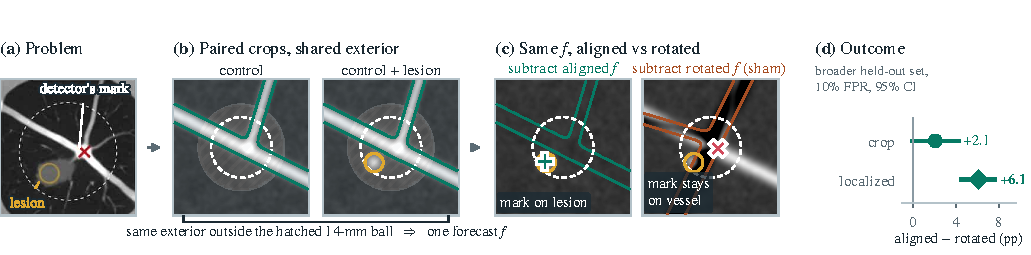
\includegraphics[width=\textwidth]{figures/overview.pdf}
\caption{Problem, design and outcome. (a)~A compact-blob search in the 10-mm core (dashed) returns the vessel junction (red cross) instead of the lesion (gold ring). (b)~A control and its lesion copy share the exterior outside the hatched 14-mm ball, so both receive the same forecast $f$. (c)~Subtracting the aligned $f$ moves the returned location to the lesion; the rotated sham leaves it on the vessel. (d)~On the broader held-out set, alignment changes crop sensitivity only slightly but raises localized sensitivity (95\% CIs). Panel (a) was created in BioRender; (b) and (c) use a generated slice whose marks are computed with a simplified readout.}
\label{fig:overview}
\end{figure*}
